\documentclass[10pt,conference]{IEEEtran}

\ifCLASSINFOpdf
	\usepackage[pdftex]{graphicx}
	%\graphicspath{{./figs/}}
	\DeclareGraphicsExtensions{.pdf,.jpeg,.png}
\else
	\usepackage[dvips]{graphicx}
	%\graphicspath{{./figs/}}
	\DeclareGraphicsExtensions{.eps}
\fi

\usepackage[cmex10]{amsmath}
\usepackage{amsfonts}
\usepackage[tight,footnotesize]{subfigure}
\usepackage{xcolor}
\usepackage[lined,ruled]{algorithm2e}
\usepackage{hyperref}
\usepackage[latin1]{inputenc}
\usepackage{tikz}
\usetikzlibrary{shapes}
\usetikzlibrary{arrows}
\usetikzlibrary{shapes.geometric}

\usepackage[]{algorithm2e}

\newtheorem{property}{Property}
\newtheorem{proposition}{Proposition}
\newtheorem{theorem}{Theorem}
\newtheorem{conjecture}{Conjecture}
\newtheorem{question}{Question}
\newtheorem{definition}{Definition}
\newtheorem{corollary}{Corollary}

\makeatletter
\pgfdeclareshape{datastore}{
\inheritsavedanchors[from=rectangle]
\inheritanchorborder[from=rectangle]
\inheritanchor[from=rectangle]{center}
\inheritanchor[from=rectangle]{base}
\inheritanchor[from=rectangle]{north}
\inheritanchor[from=rectangle]{north east}
\inheritanchor[from=rectangle]{east}
\inheritanchor[from=rectangle]{south east}
\inheritanchor[from=rectangle]{south}
\inheritanchor[from=rectangle]{south west}
\inheritanchor[from=rectangle]{west}
\inheritanchor[from=rectangle]{north west}
\backgroundpath{
    %  store lower right in xa/ya and upper right in xb/yb
\southwest \pgf@xa=\pgf@x \pgf@ya=\pgf@y
\northeast \pgf@xb=\pgf@x \pgf@yb=\pgf@y
\pgfpathmoveto{\pgfpoint{\pgf@xa}{\pgf@ya}}
\pgfpathlineto{\pgfpoint{\pgf@xb}{\pgf@ya}}
\pgfpathmoveto{\pgfpoint{\pgf@xa}{\pgf@yb}}
\pgfpathlineto{\pgfpoint{\pgf@xb}{\pgf@yb}}
 }
}
\makeatother

\newcommand{\riham}[1]{{\color{red}{#1}}}
\newcommand{\james}[1]{{\color{blue}{#1}}}


\begin{document}

% Define block styles
\tikzstyle{block} = [rectangle, draw, fill=blue!20, 
    text width=8em, text centered, rounded corners, minimum height=6em, node distance=4cm]
\tikzstyle{line} = [draw, -latex']

\title{Cores Decomposition of Networks - Fall 2018}
\author{
\IEEEauthorblockN{Akshay Aggarwal}
\IEEEauthorblockA{Department of Computer Science, Rutgers University\\ Piscataway, NJ, USA\\
Email: akshay.aggarwal@rutgers.edu}
}

\maketitle
\begin{abstract}
\textnormal{
The k-core decomposition of a network is an algorithm to reveal the hierarchical structure of large networks by partitioning them into smaller 'cores'. In this project, we implement and visualize the two models of this algorithm based on 1) The degree of nodes and 2) The weights of the edges of the nodes, and then extract each layer of resulting graph and visualize them as well. The interface is a website where users can view and interact with graphs representing networks and see information on the computation performed on these graphs.
}
\end{abstract}
%\onecolumn \maketitle \normalsize \vfill

\IEEEpeerreviewmaketitle
%%%%%%%%%%%%%%%%%%%%%%%%%%%%%%%%%%%%%%%%%%%%%%%%%%%%%%%%%%%%%%%%%%%%%%%%%%%%%%%%%%%%%%%%%%%%%%%%%%%%%%%%%
\section{Project Description}\label{sec:1. Project Description}
%%%%%%%%%%%%%%%%%%%%%%%%%%%%%%%%%%%%%%%%%%%%%%%%%%%%%%%%%%%%%%%%%%%%%%%%%%%%%%%%%%%%%%%%%%%%%%%%%%%%%%%%%
\textnormal{
The k-core decomposition of a network helps us in finding the cohesive groups of nodes within that network. A cohesive group can be defined as the group of nodes with strong interconnections between them. This can help identify, for example, groups of countries with the strongest trade connections or the most connected group of airports. This algorithm will reveal such groups in a hierarchical manner and then visualize the resulting groups found in the network. This project provides insight into the working of the algorithm along with its computation time based on the size of the input graph. The $k^{th}$ core of a graph can be described as the group of vertices where each vertex has degree at least $k$. A layer is defined as a sub-graph of the network which contains only the edges which fall in the highest core induced by the algorithm.\\
}

The project has four stages: Gathering, Design, Infrastructure Implementation, and User Interface.

%\subsection{Stage1 - The Requirement Gathering Stage. } \label{sec:1	Requirement Gathering Stage. } 
%\begin{itemize} 
\item{A general description:
Suppose we have a network of countries with trade deals between them represented as a graph. An edge between country A and country B represents a trade deal between the two countries. Now we want to find the sub-groups of countries with the maximal trade deals between them. We can run the k-core decomposition to find the sub-graph containing these countries. All the countries which have an edge between them and fall into the highest core can then be extracted as a layer. Now, say, we want to say the countries which have the maximal trade deals once the if the above countries had no trade deals between them. We will can then remove the edges between the above countries and run the k-core decomposition algorithm on the resulting graph again to find this new group of countries. The edges which fall into these groups are now the next layer of the network. 
} 

\item{User 1: } Learner
\item{Learner - Interaction Modes: }
Read page and play visualizations on given examples.
\item{Learner - Scenarios: }
	\begin{itemize} 
	\item{Scenario1 description: }
	A student is going to learn the k-core decomposition algorithm. The student can read the algorithm description and go through the interactive visualization of the algorithm on preset input. The student can then see how the size and density of the graph affects the computation time and concentration of edges in each layer of the graph and hence develop a better understanding of the algorithm.
	\item{System Data Input for Scenario 1: }
	The input is the selection of inputs given on the web site. 
    \item{Input Data Types for Scenario 1:}
    The pre-generated graphs can be selected from a list.
	\item{System Data Output for Scenario 1: }
	The website tool generates the visualization of the cores and subsequent layers of the graph.
    \item {Output Data Types for Scenario 1: }
    The output is a graph with the cores represented by colors as well as tool tips as layers generated in separate sections below the main graph.
    \item{Scenario 2 description:}
	An individual has seen or learned about the algorithm previously, but needs a quick refresher on how the algorithm works. They will just run a single preset and not fiddle with parameters.
	\item{System Data Input for Scenario 2: }
	The individual selects the graph they want to run it on.
    \item{Input Data Types for Scenario 2:}
    The user clicks on a preset on the preset list.
	\item{System Data Output for Scenario 2: }
    The individual sees the algorithm working over the graph and the resulting cores.
    \item {Output Data Types for Scenario 2: }
    Visualizations occur in UI elements on the webpage. The cores are represented by the colors and the layers are visualized. The computation time and edge concentration for each layer are also visualized.
	\end{itemize}
\item{User 2: } Teacher
\item{Teacher - Interaction Modes: }
Play visualizations on given examples and specialized examples which they input.
\item{Teacher - Scenarios: }
	\begin{itemize} 
	\item{Scenario 1 description:}
	A teacher would like an interactive, visual accompaniment to their lecture on the core decomposition. 
	\item{System Data Input for Scenario 1: }
	The teacher can select one of the preset graphs to run the algorithm on, or they can generate their own graphs as well with the accompanied graph generator program.
    \item{Input Data Types for Scenario 1:}
    The teacher can specify the number of nodes and edges desired in the graph to be processed to the random graph generator program. 
	\item{System Data Output for Scenario 1: }
	A random graph generated, which is then processed by the k-cores program and the resulting file is visualized using the web-tool.
    \item {Output Data Types for Scenario 1: }
    The graph generator outputs the graph as an adjacency list. The output from the k-cores algorithm is a JSON file which can be used with the web-tool.
    \item{Scenario 2 description:}
	The teacher does not have time to cover the algorithm in class, but wants students to learn it. They direct students to the web tool site for them to tinker with the algorithm themselves based on some graphs pre-generated by the teacher.
	\item{System Data Input for Scenario 2: }
	The teacher can specify specific inputs to run on or direct students to play around with example or even their own inputs.
    \item{Input Data Types for Scenario 2:}
    A special link to a web-page loaded with the teacher's desired presets generated by the graph generator program.
	\item{System Data Output for Scenario 2: }
	Each of the teacher's students see the visualization of the algorithm along with the k-cores in the graph and the subsequent layers extracted from the graph.
    \item {Output Data Types for Scenario 2: }
    Interactive visualizations along with graphs representing the computation time and edge concentration for each layer.
	\end{itemize}
\item{User 3: } A user who needs to analyze a network.
\item{User - Interaction Modes: }
Run the algorithm on specialized examples which they input. Download the resulting rankings to their computer.
\item{User - Scenarios: }
	\begin{itemize} 
	\item{Scenario 1 description:}
	An individual would like to quickly run the algorithm on a small dataset without having to write code or import a library.
	
	\item{System Data Input for Scenario1: }
	The individual would input the specific graph for which they want to run the algorithm on and will specify the graph explicitly.
    \item{Input Data Types for Scenario 1:}
    The user can input a raw text file containing the graph represented as an adjacency list.
	\item{System Data Output for Scenario 1: }
	
    \item {Output Data Types for Scenario 1:}
    The JSON files of the main graph and each layer which contain the distinct cores and can be run using the web-tool and the graph can be visualized and analyzed for the edge concentration in layers and computation time.
    \item{Scenario 2 description: Visualizing a particular layer of a very large graph}
	An individual would like to analyze only a particular layer extracted from a very large graph ($order of edges > 2^{10}$).
	\item{System Data Input for Scenario 2: }
	The individual explicitly defines a graph as an adjacency list and runs the algorithm on it. The \textit{Large Graphs} section of the web-tool can be used to visualize individual layers.
    \item{Input Data Types for Scenario 2:}
    A random graph can be generated by inputting the number of nodes and edges desired in the graph or a graph can be input as an adjacency list to the program.
	\item{System Data Output for Scenario 2: }
	The user obtains the file containing the core number and the files for each layer along with the files containing the information on the concentration of edges and computation time for each of them. These files can then be visualized.
    \item {Output Data Types for Scenario 2:}
    JSON files containing the data that can be visualized using the \textit{Large Graphs} section of the website. 
	\end{itemize}
\end{itemize}
\subsection{Stage1 - The Requirement Gathering Stage. }\label{sec:1 Requirement Gathering Stage. }
%%%%%%%
\begin{itemize} 
\item{A general description:
Suppose we have a network of countries with trade deals between them represented as a graph. An edge between country A and country B represents a trade deal between the two countries. Now we want to find the sub-groups of countries with the maximal trade deals between them. We can run the k-core decomposition to find the sub-graph containing these countries. All the countries which have an edge between them and fall into the highest core can then be extracted as a layer. Now, say, we want to say the countries which have the maximal trade deals once the if the above countries had no trade deals between them. We will can then remove the edges between the above countries and run the k-core decomposition algorithm on the resulting graph again to find this new group of countries. The edges which fall into these groups are now the next layer of the network. 
} 

\item{User 1: } Learner
\item{Learner - Interaction Modes: }
Read page and play visualizations on given examples.
\item{Learner - Scenarios: }
	\begin{itemize} 
	\item{Scenario1 description: }
	A student is going to learn the k-core decomposition algorithm. The student can read the algorithm description and go through the interactive visualization of the algorithm on preset input. The student can then see how the size and density of the graph affects the computation time and concentration of edges in each layer of the graph and hence develop a better understanding of the algorithm.
	\item{System Data Input for Scenario 1: }
	The input is the selection of inputs given on the web site. 
    \item{Input Data Types for Scenario 1:}
    The pre-generated graphs can be selected from a list.
	\item{System Data Output for Scenario 1: }
	The website tool generates the visualization of the cores and subsequent layers of the graph.
    \item {Output Data Types for Scenario 1: }
    The output is a graph with the cores represented by colors as well as tool tips as layers generated in separate sections below the main graph.
    \item{Scenario 2 description:}
	An individual has seen or learned about the algorithm previously, but needs a quick refresher on how the algorithm works. They will just run a single preset and not fiddle with parameters.
	\item{System Data Input for Scenario 2: }
	The individual selects the graph they want to run it on.
    \item{Input Data Types for Scenario 2:}
    The user clicks on a preset on the preset list.
	\item{System Data Output for Scenario 2: }
    The individual sees the algorithm working over the graph and the resulting cores.
    \item {Output Data Types for Scenario 2: }
    Visualizations occur in UI elements on the webpage. The cores are represented by the colors and the layers are visualized. The computation time and edge concentration for each layer are also visualized.
	\end{itemize}
\item{User 2: } Teacher
\item{Teacher - Interaction Modes: }
Play visualizations on given examples and specialized examples which they input.
\item{Teacher - Scenarios: }
	\begin{itemize} 
	\item{Scenario 1 description:}
	A teacher would like an interactive, visual accompaniment to their lecture on the core decomposition. 
	\item{System Data Input for Scenario 1: }
	The teacher can select one of the preset graphs to run the algorithm on, or they can generate their own graphs as well with the accompanied graph generator program.
    \item{Input Data Types for Scenario 1:}
    The teacher can specify the number of nodes and edges desired in the graph to be processed to the random graph generator program. 
	\item{System Data Output for Scenario 1: }
	A random graph generated, which is then processed by the k-cores program and the resulting file is visualized using the web-tool.
    \item {Output Data Types for Scenario 1: }
    The graph generator outputs the graph as an adjacency list. The output from the k-cores algorithm is a JSON file which can be used with the web-tool.
    \item{Scenario 2 description:}
	The teacher does not have time to cover the algorithm in class, but wants students to learn it. They direct students to the web tool site for them to tinker with the algorithm themselves based on some graphs pre-generated by the teacher.
	\item{System Data Input for Scenario 2: }
	The teacher can specify specific inputs to run on or direct students to play around with example or even their own inputs.
    \item{Input Data Types for Scenario 2:}
    A special link to a web-page loaded with the teacher's desired presets generated by the graph generator program.
	\item{System Data Output for Scenario 2: }
	Each of the teacher's students see the visualization of the algorithm along with the k-cores in the graph and the subsequent layers extracted from the graph.
    \item {Output Data Types for Scenario 2: }
    Interactive visualizations along with graphs representing the computation time and edge concentration for each layer.
	\end{itemize}
\item{User 3: } A user who needs to analyze a network.
\item{User - Interaction Modes: }
Run the algorithm on specialized examples which they input. Download the resulting rankings to their computer.
\item{User - Scenarios: }
	\begin{itemize} 
	\item{Scenario 1 description:}
	An individual would like to quickly run the algorithm on a small dataset without having to write code or import a library.
	
	\item{System Data Input for Scenario1: }
	The individual would input the specific graph for which they want to run the algorithm on and will specify the graph explicitly.
    \item{Input Data Types for Scenario 1:}
    The user can input a raw text file containing the graph represented as an adjacency list.
	\item{System Data Output for Scenario 1: }
	
    \item {Output Data Types for Scenario 1:}
    The JSON files of the main graph and each layer which contain the distinct cores and can be run using the web-tool and the graph can be visualized and analyzed for the edge concentration in layers and computation time.
    \item{Scenario 2 description: Visualizing a particular layer of a very large graph}
	An individual would like to analyze only a particular layer extracted from a very large graph ($order of edges > 2^{10}$).
	\item{System Data Input for Scenario 2: }
	The individual explicitly defines a graph as an adjacency list and runs the algorithm on it. The \textit{Large Graphs} section of the web-tool can be used to visualize individual layers.
    \item{Input Data Types for Scenario 2:}
    A random graph can be generated by inputting the number of nodes and edges desired in the graph or a graph can be input as an adjacency list to the program.
	\item{System Data Output for Scenario 2: }
	The user obtains the file containing the core number and the files for each layer along with the files containing the information on the concentration of edges and computation time for each of them. These files can then be visualized.
    \item {Output Data Types for Scenario 2:}
    JSON files containing the data that can be visualized using the \textit{Large Graphs} section of the website. 
	\end{itemize}
\end{itemize}

\subsection{Stage2 - The Design Stage. }\label{sec: 2:The Design Stage.}
%%%%%%%%%%%%%%%%%%%%%%%%%%%%%%%%%%%%%%%%%%%%%%%%%%%%%%%%%%%%%%%%%%%%%%%%%%%%%%%%%%%%%%%%%%%%%%%%%%%%%%%%%%
\begin{itemize} 
\item{Project Flow: }
    \begin{enumerate}
        \item The user explicitly inputs a graph G OR graph G is generated using the Graph Generator Program.
        \item Graph G is input to the $U_{k-core}$ (unweighted k-core) or to the $W_{k-core}$ (weighted k-core) algorithm.
        \item The top layer is extracted from the output of the k-core algorithm. The new graph $G' = (V,E')$ where $E' = E-E*$ is fed back into step 2.
        \item Steps 2 and 3 are repeated till all the layers are extracted and $|E'| = 0$.
        \item The resultant layers, their computation time and concentration of edges in each layer is visualized using the website. 
    \end{enumerate}

\end{itemize}

 \begin{itemize}
\item{ Flow Diagram. } \\
    \begin{tikzpicture}[node distance = 2cm, auto]
    	\node [block] (graph_input) {1.Explicitly Input graph G};
        \node [block, right of=graph_input] (generate_graph) {1. Randomly Generate Graph G};
        \node [block, below of=graph_input] (unweighted_kcore) {2. Perform $U_{k-core}$ on G};
        \node [block, right of=unweighted_kcore] (weighted_kcore) {2. Perform $W_{k-core}$ on G};
        \node [block, below of=unweighted_kcore] (extract_layers) {3. Extract Layer and computation-time value, edge concentration value};
        
        \node [draw, diamond,, aspect=2, node distance = 4cm, fill=blue!20, below of=extract_layers] (layer_decision) {4. $|E'| = 0?$ };
        
        \node [block, below of= layer_decision] (visualize) {5. Visualize using website};
        
        \path[every node/.style={sloped,anchor=south,auto=false}]
        (graph_input) [->, thick] edge node [below] {} (unweighted_kcore)
        (graph_input) [->, thick] edge node [below] {} (weighted_kcore)
        (generate_graph) [->, thick] edge node [below] {} (unweighted_kcore)
        (generate_graph) [->, thick] edge node [below] {} (weighted_kcore)
        (unweighted_kcore) [->, thick] edge node [below] {} (extract_layers)
        (weighted_kcore) [->, thick] edge node [below] {} (extract_layers)
        (extract_layers) [->, thick] edge node [below] {} (layer_decision)
        (layer_decision) [->, thick] edge [bend right=45] node {No} (unweighted_kcore)
        (layer_decision) [->, thick] edge [bend right] node [above] {No} (weighted_kcore)
        (layer_decision) [->, thick] edge node [below] {Yes} (visualize);
    \end{tikzpicture}
    
\item{ High Level Pseudo Code System Description. } \\
\LinesNumbered
\begin{algorithm}
 \KwIn{$|V|, |E|$}
 \KwOut{Graph $(V,E)$}
 $n \gets 0$ \\
 \While {$n \neq |E|$}{
     $u \gets rand \mod |V|$  \\
     $v \gets rand \mod |V|$ \\
     $e \gets (u,v)$ \\
     \If{$e \not\in{E}$}{
        $E \cup e$ \\
        $n \gets n+1$
       
     }
 }
 
 \caption{Generate Graph}
 \end{algorithm}
 
\begin{algorithm}
 
\KwIn{Graph G = (V, E) as an adjacency list}
\KwOut{Array $deg$ with core number for each vertex}

compute the degrees of vertices \\
order the set of vertices V \\
in increasing order of their degrees \\
\ForEach {$v \in V$ in the order} {
    $core[v] \gets degree[v]$ \\
    \ForEach{$u \in Neighbours(v)$} {  
        \If {degree[u] $>$ degree[v]} {
            $degree[u] \gets degree[u] $-$ 1$   \\
            reorder V accordingly
        }
    }
}
\caption{Unweighted k-core Algorithm}
\end{algorithm}


\begin{algorithm}
 
\KwIn{Graph G = (V, E) as an adjacency list}
\KwOut{Array $deg$ with core number for each vertex}

computer weighted degrees of vertices  \\
order the set of vertices V \\
in increasing order of their degrees \\
\ForEach {$v \in V$ in the order} {
    $core[v] \gets degree[v]$ \\
    \ForEach{$u \in Neighbours(v)$} {  
        \If {degree[u] $>$ degree[v]} {
            $degree[u] \gets degree[u] $-$ w_{ij}$  \\
            reorder V accordingly
        }
    }
}
\caption{Weighted k-core Algorithm}
\end{algorithm}

\begin{algorithm}
 
\KwIn{Graph $G = (V, E)$ as an adjacency list, Graph $G^* = (V,E^*)$ containing the edges in the highest core.}
\KwOut{Graph $G_R = (V, E_R)$}

\ForEach {$e \in E$} {
    \If {$e \in E^*$} {
       $E \gets E$-$e$   \\
    }
}
\caption{Layer Extraction}
\end{algorithm}

\begin{algorithm}
  \KwIn{Graph $(V,E)$ }
 \For{$(u,v) \in{E}$}{
   $d \gets$ distance from $u$ to $v$ \\
   $f_x, f_y \gets springForce(d, alpha)$ \\
   Add $f_x$ to $u.xVelocity$ and $v.xVelocity$ \\
   Add $f_y$ to $u.yVelocity$ and $v.yVelocity$ 
 }
 \For{$ v\in{V}$}{
   $f_x, f_y \gets repulsionForce(v, V, alpha)$ \\
   $v.xVelocity \gets v.xVelocity + f_x$ \\
   $v.yVelocity \gets v.yVelocity + f_y$
 }
 \For{$ v\in{V}$}{
   $v.x \gets v.x + v.xVelocity$ \\
   $v.y \gets v.y + v.yVelocity$
 }
 \caption{Tick in Simulation}
\end{algorithm}

\item The algorithms are as follow:
\begin{itemize}
\setlength\itemsep{1em}
    \item{\textit{The graph generator:}}
    Given input $n,m$ the graph generator will generate a graph $G=(v,E)$ as an adjacency list where $|V| = n$ and $|E| = m$. For each vertex $v \in V$, the neighbors are represented as a unique $set$. To generate an edge, the function performs the following steps:
    \begin{enumerate}
        \item Set $count=0$.
        \item Randomly pick $u$ and $v$ from $V$.
        \item Try to insert $v$ in the adjacency set of $u$. If edge $(u,v) \in E$ then go back to step 2.
        \item Else $E = E\cup (u,v)$.
        \item Increment $count$. If $count \neq m$ then go back to step 2.
    \end{enumerate}
    The $set:insert$ step takes $O(\log{n})$ time.
    
    \item{\textit The k-core Algorithm:}
    The k-Core algorithm is as follow:
    \begin{enumerate}
        \item Create an array $deg$ of size $|V|$ representing the vertices in $V$.
        \item For each vertex, assign the value of $deg[u]$ as follow:
        \begin{itemize}
            \item{\textit{Unweighted}}
            Degree of vertext $u$.
            \item{\textit{Weighted}} 
            $k_u$, the weighted degree of vertex $u$ where $k_u = \sum w_{u,v}$ where $w_{u,v}$ is the weight of the edge $(u,v)$.
        \end{itemize}
        \item Sort the vertices in increasing order of their degrees.
        \item For $k \in [0,1,2,...,md]$ where $md$ is the maximum degree in the array $deg$, for each vertex $u$ of degree $k$, for each $v \in Neighbours(u)$, do:
        \begin{itemize}
            \item{\textit{Unweighted}}
            If $deg[v] > deg[u]$ then delete edge $(v,u)$ and decrement $deg[v]$.
            \item{\textit{Weighted}}
            If $deg[v] > deg[u]$ then delete edge $(v,u)$ and $deg[v] = deg[v] - w_{v,u}$.
            \newline If $deg[v] - w_{v,u} < k$, then  $deg[v] = k$.
        \end{itemize}
        \item The array $deg$ will contain the core numbers for each $v \in V$.
    \end{enumerate}
    The sorting of degrees can be performed in $O(|V|)$ time using \textit{bucket sort}. Step 3 takes $O(|E|)$ time.
\end{itemize}
\end{itemize}



\subsection{Stage3 - The Implementation Stage. }\label{sec: 3 The Implementation Stage.}
%%%%%%%%%%%%%%%%%%%%%%%%%%%%%%%%%%%%%%%%%%%%%%%%%%%%%%%%%%%%%%%%%%%%%%%%%%%%%%%%%%%%%%%%%
\textnormal{
The generation of random graphs and implementation and execution of the algorithms is performed using C++ in Microsoft Visual Studio. For the interactive website, JavaScript, HTML5 and CSS are used. The library used is D3.js (data-driven-documents).
%Building the corresponding relational tables, according to the proposed ER model described in the previous phase %enforcing the different integrity constraints.  
The deliverables for this stage include the following items:
\begin{itemize} 
\item{}
The size of the graphs generated are from 64 vertices till 4096 vertices, for convenience, with the following relations between the nodes and edges:
    \begin{itemize}
        \item $ |E| = |V|/2 $
        \item $ |E| = |V| $
        \item $ |E| = 2|V| $
        \item $ |E| = |V|\log |V|$
    \end{itemize}
The graph generator program selects two nodes $u$ and $v$ where the uniform probability of a node being picked is $\frac{1}{|V|}$ and checks if an edge already exists between the two nodes. If the edge does not exist, it is added to $E$.
    \begin{itemize}
        \item For weighted graphs, the link weight between nodes $u$ and $v$ is defined as: 
        $$w_{u,v} = size(Neighbours(u) \cup Neighbours(v))$$
    \end{itemize}
%The SQL tables that represent the ER project model, along with at least 3-5 rows of concrete data per table.
\item{}
The k-core algorithm program which extracts the layers in the graph and writes the computation times and number of edges for each layer to a JSON file format.
%The normalization steps for each table, along with explanations/justifications of each normalization step.
\item{}
A website which visualizes the generated files.
%The SQL table after the normalization steps (showing all table attributes).
\item{}
Demo and sample findings
%The SQL statements used to create the SQL tables, including the required triggers as well as the integrity constraints. At %least 2 triggers and 2 of each of the following constraint types have to exist in the project tables overall: 
\begin{itemize} 
\item{}
    	Data size: In terms of  RAM size;  Disk Resident?; Streaming ?;  
    \item{}
    	List the most interestng findings in the data if it is a Data Exploration Project. For other project types consult with your project supervisor what the corresponding outcomes shall be. Concentrate on demonstrating the Usefuness and Novelty of your application.
    %Whether some users will be denied access and/or updates to some data according to their roles (for example: student1 %can not access other students' ' grades, so a violation error pops up upon that action. Another example: a sales person %can see an item price, but can not change it, since only a manger can, also a violation error pops up upon that update %attempt).
\end{itemize}
\end{itemize}
}


\subsection{Stage4 -	User Interface. }\label{sec: 4. User Interface.}
%%%%%%%%%%%%%%%%%%%%%%%%%%%%%%%%%%%%%%%%%%%%%%%%%%%%%%%%%%%%%%%%%%%%%%%%%%%%%%%%%%%%%%%%%%%%%%%%%%%%%%%%%%
The user interface is as follow:
\begin{itemize}
    \item{\textit{The Main Page:}} 
    \begin{figure}[!htbp]
    \begin{center}
    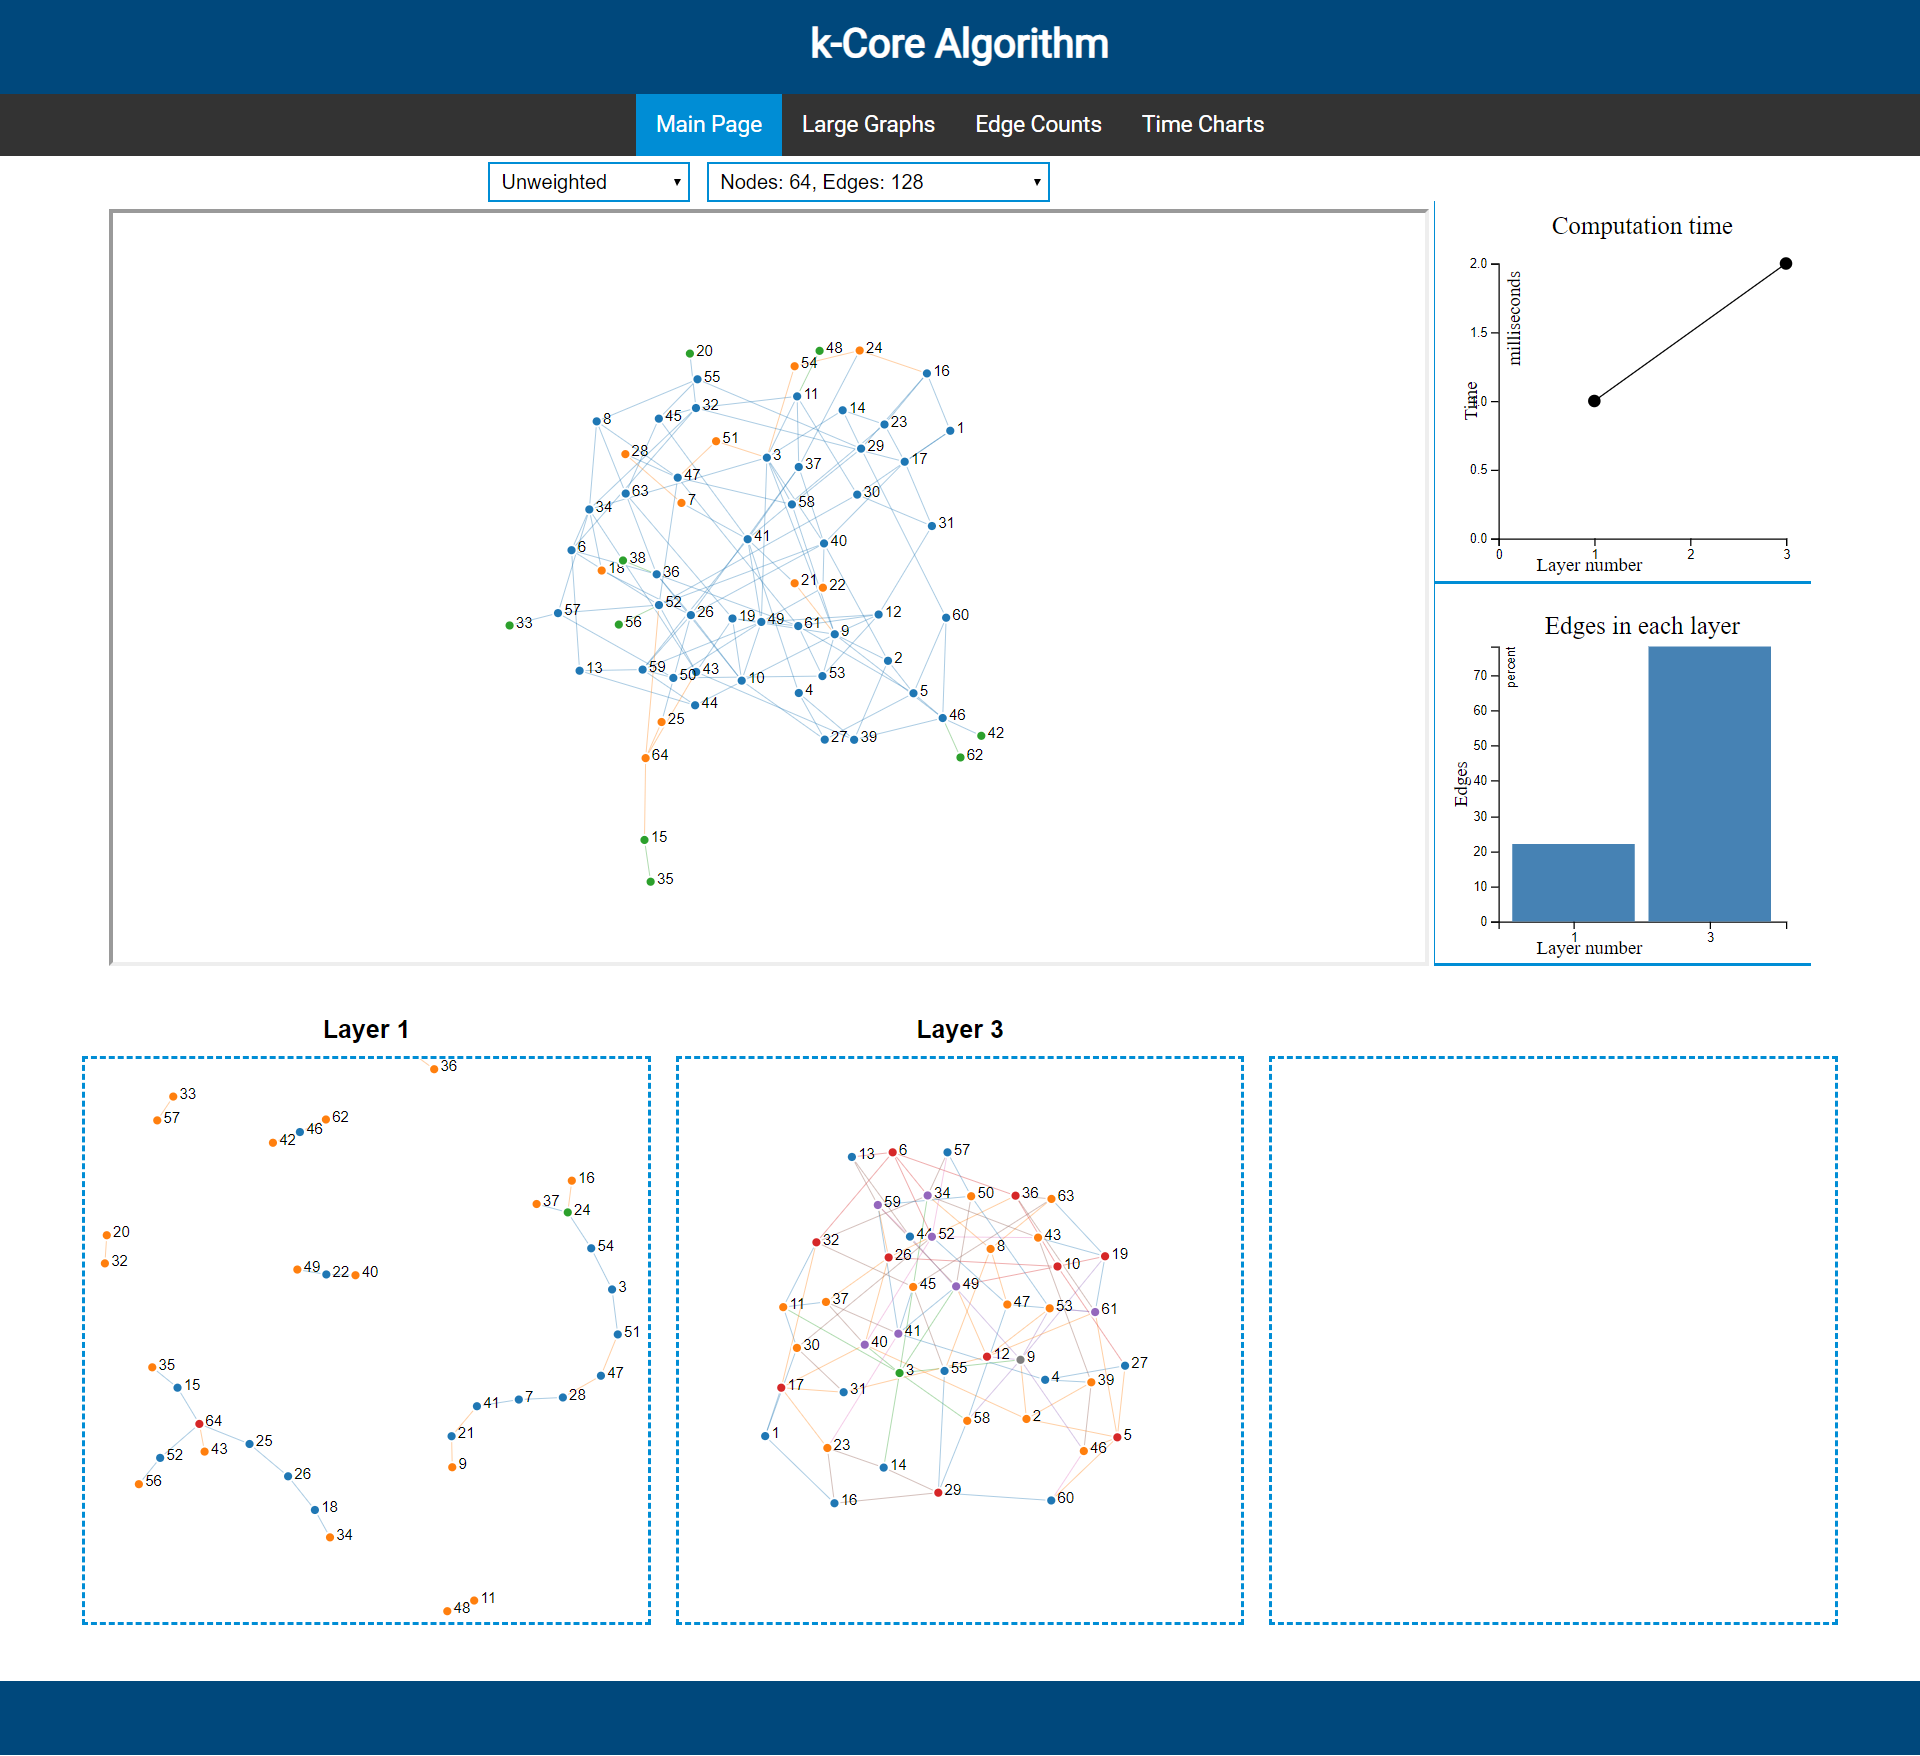
\includegraphics[width=8cm]{Final_Interface.png}
    \end{center}
    \caption{ The Main page }
    \end{figure}
    \begin{itemize}
        \item The user has the option of selecting whether they want to see the weighted graphs or the unweighted graphs. Once selected, the desired node size and edge counts can be selected from a second selector.
        \item Once a graph is selected, the corresponding bar chart depicting the concentration of edges in each layer and the computation time for each layer are displayed in a sidebar.
        \item The layers of the graph can be viewed by pressing the \textit{Layers} button at the bottom. 3 layers are generated at a time and the \textit{More Layers} button can be be pressed to generate further layers. The button will be available as long as there are further layers to be generated.
        \item When the \textit{mouseOver} action is performed on a vertex, all the neighbouring vertices of that vertex are highlighted and the remaining vertices are blurred out.
        \item When hovering over a vertex in the main graph, the core number of that vertex is shown.
        \item The graph vertices can be dragged within the graph container to better view a link or a vertex at the convenience of the user.
        \item A zoom function is also available on scroll-in/scroll-out for the user to focus on a vertex, a particular part of the graph or the graph as a whole.
    \end{itemize}
    
    \begin{figure}[!htbp]
    \begin{center}
    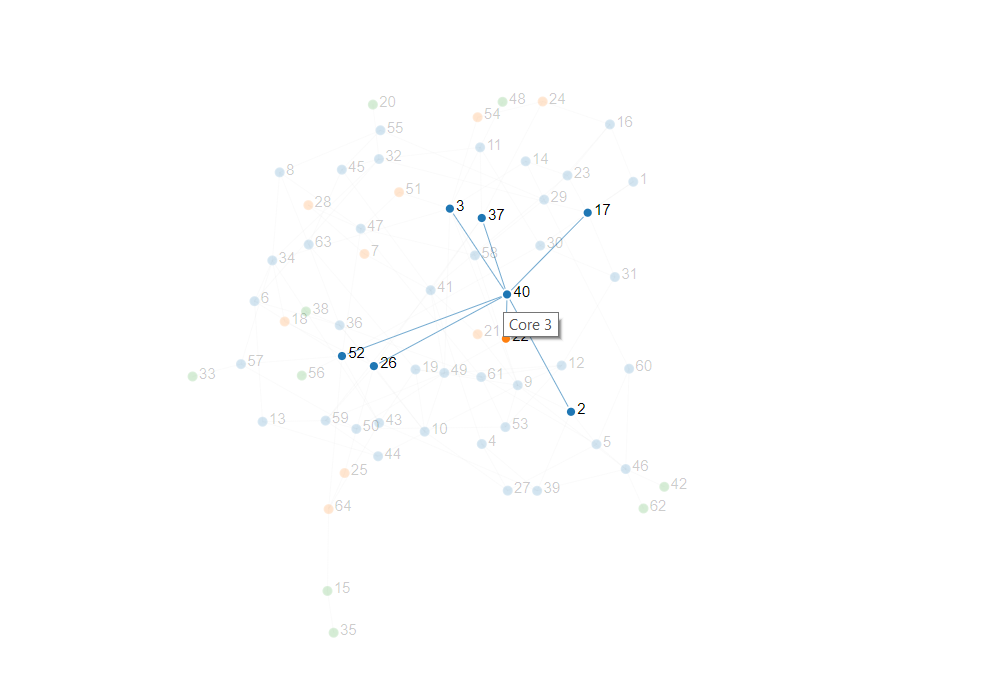
\includegraphics[width=8cm]{MouseHover.png}
    \end{center}
    \caption{ The MouseOver Effect }
    \end{figure}
    
    \begin{figure}[!htbp]
    \begin{center}
    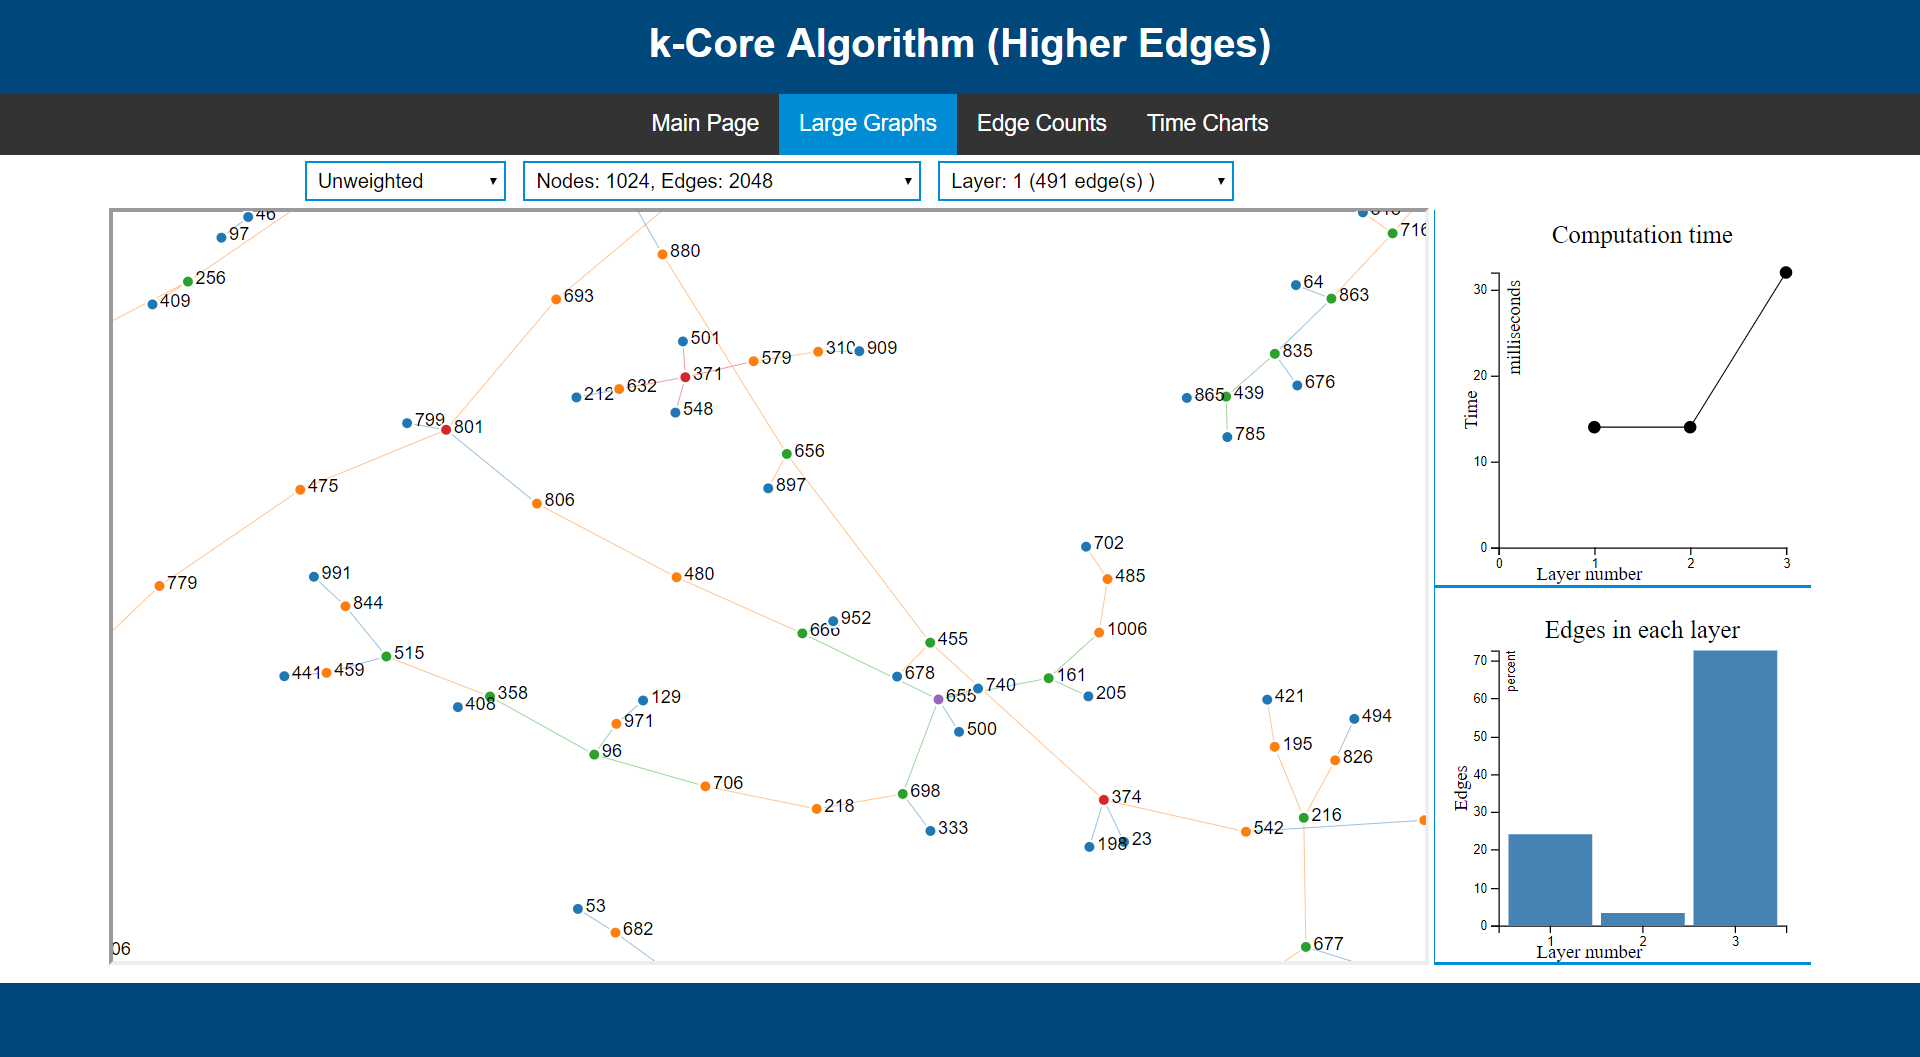
\includegraphics[width=8cm]{Large_Graphs.png}
    \end{center}
    \caption{ The Large Graphs Page }
    \end{figure}
    
    \item{\textit{Large Graphs Page:}}
    A graph with a large number of edges (in this case, $> 1024$) will have a large number of layers, and higher layers will also contain a large number of edges. To make it easier for the D3.js library to process these graphs and for the user to be able to view one layer at a time, a separate page is provided where these graphs and their layers can be viewed.
    \begin{itemize}
        \item The user can select between weighted and unweighted graphs.
        \item The user can then select the desired number of nodes and edges. The time-plot and edge concentration bar-graph will be displayed in the sidebar.
        \item When the graph is selected from the secondary drop down menu, a third selector will provide the choices of the graph's layers and also display the number of edges each of those graphs contain.
    \end{itemize}
        
    % \begin{figure}[!htbp]
    % \begin{center}
    % 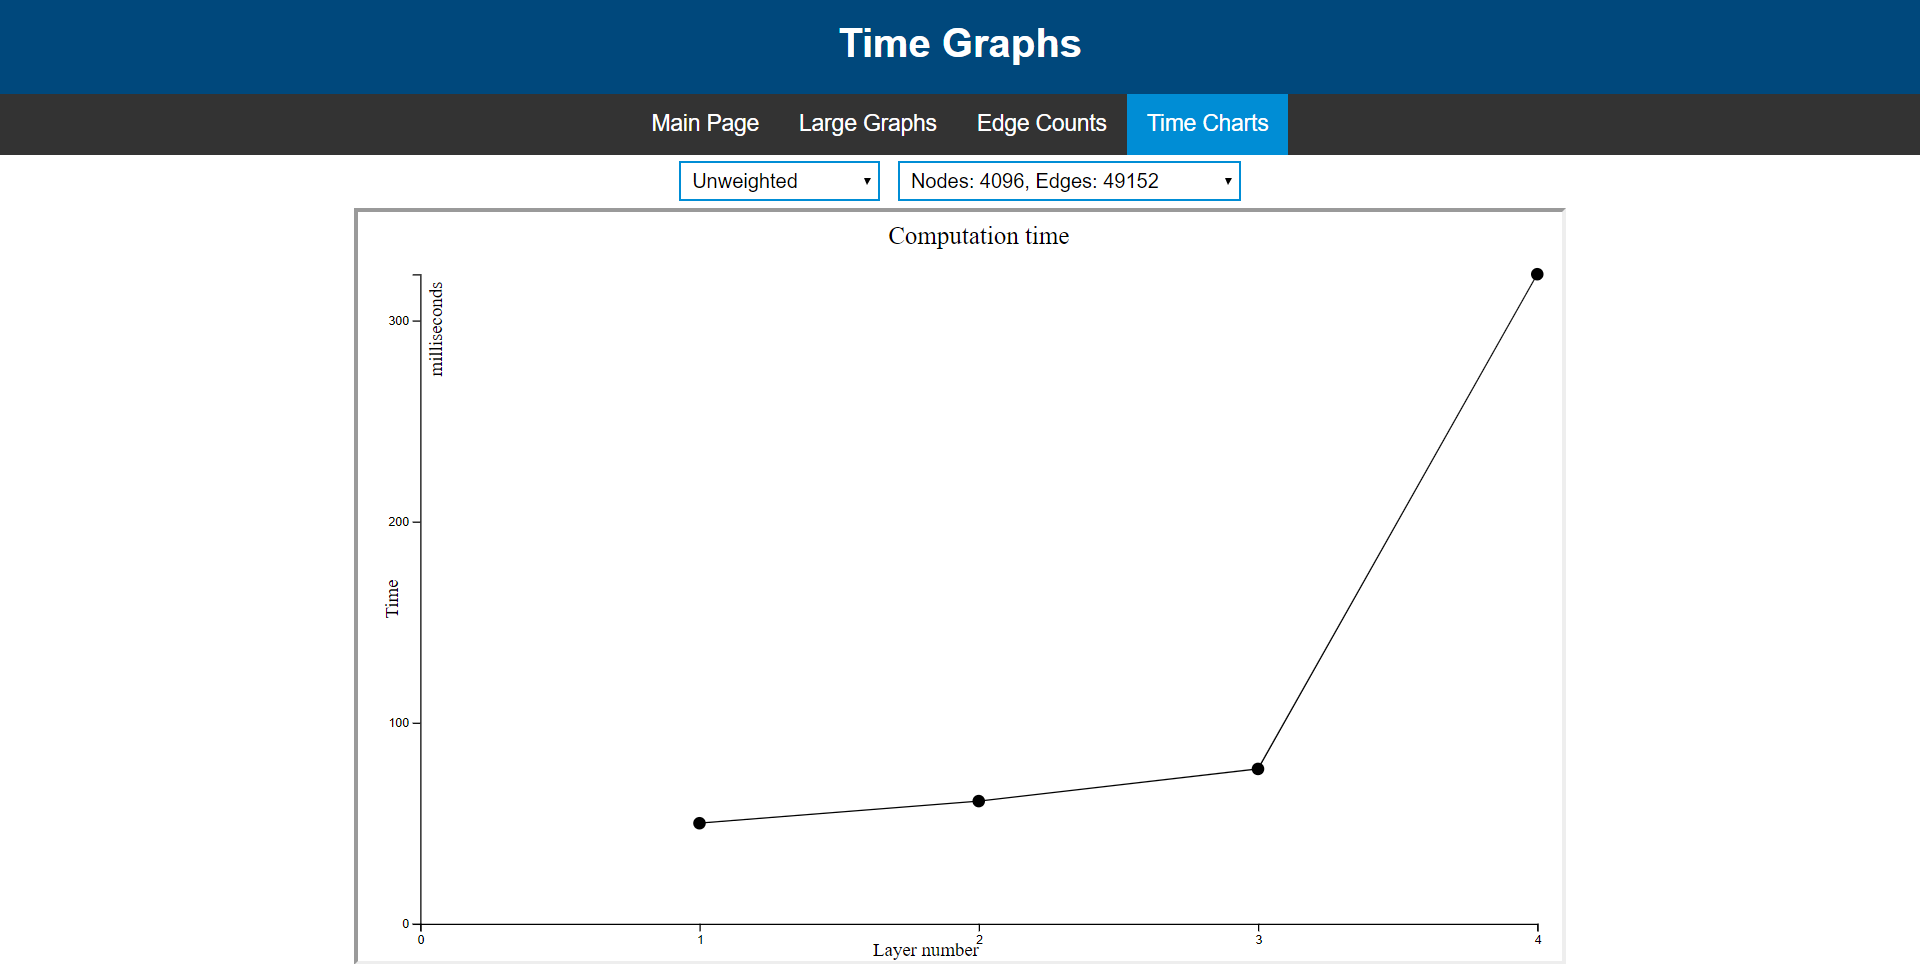
\includegraphics[width=8cm]{Time_Chart.png}
    % \end{center}
    % \caption{ The Time Plot }
    % \end{figure}
    
    % \begin{figure}[!htbp]
    % \begin{center}
    % 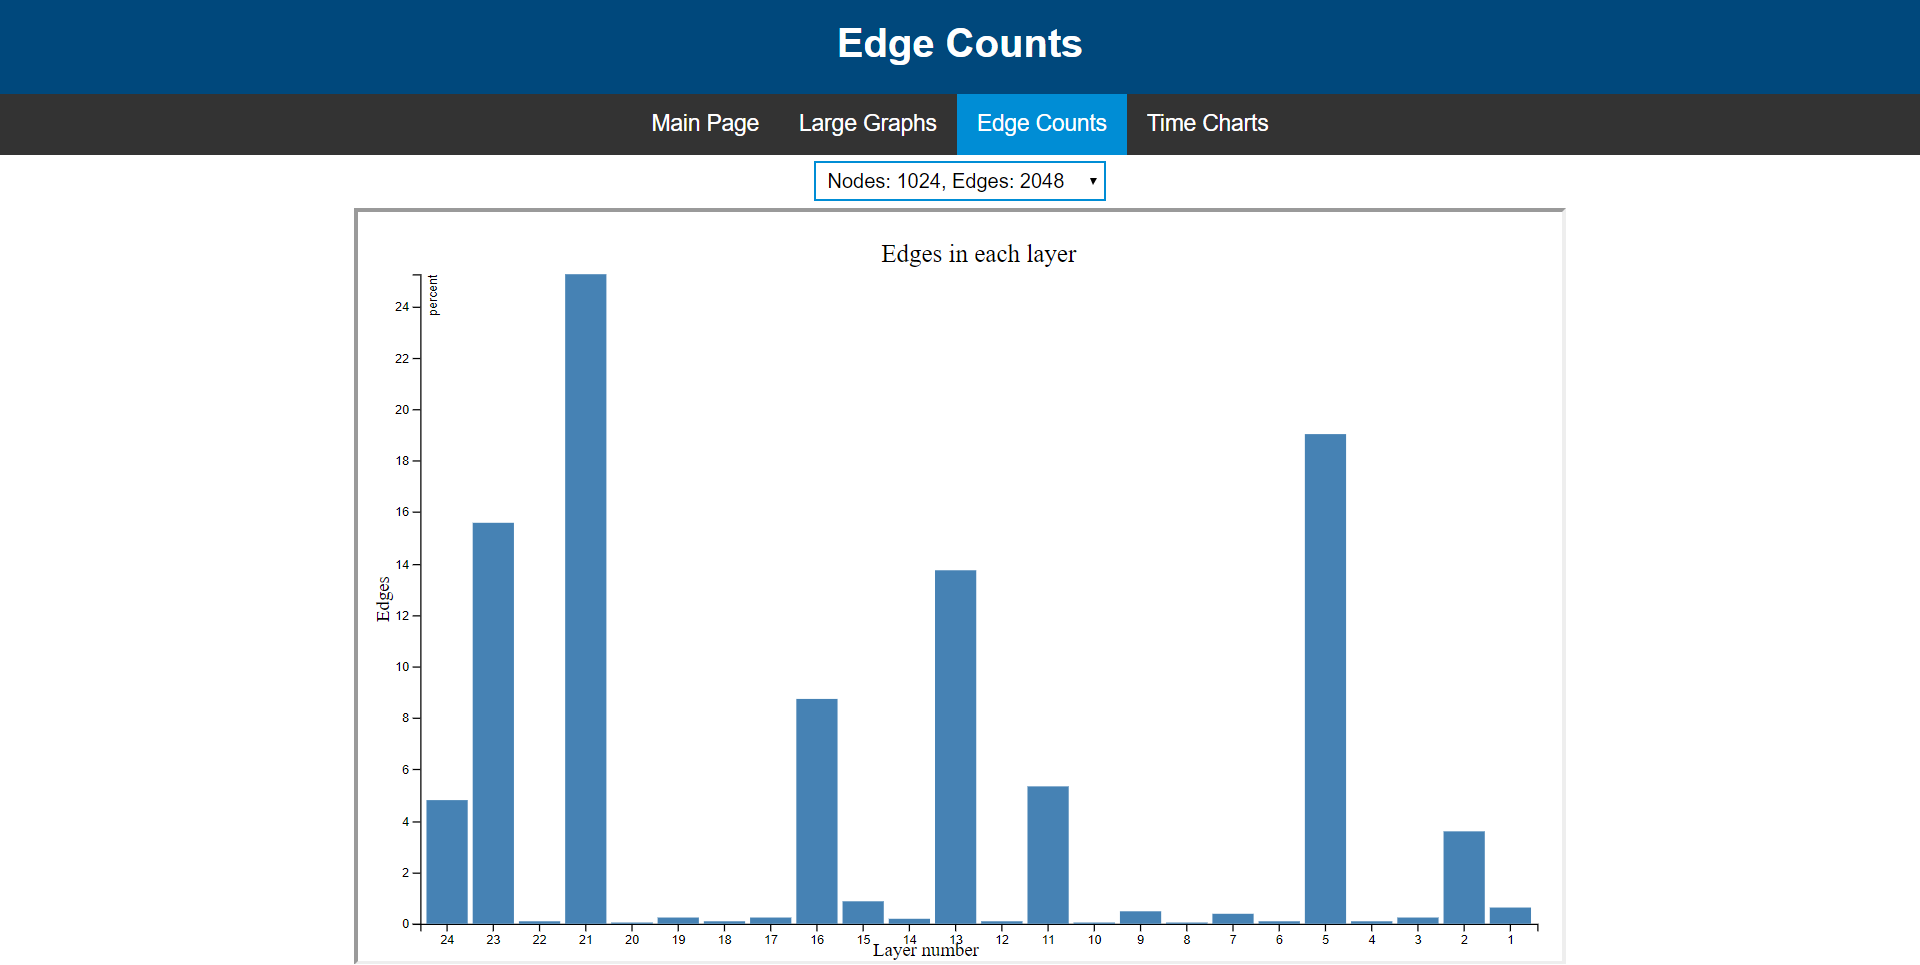
\includegraphics[width=8cm]{Edge_Concentration.png}
    % \end{center}
    % \caption{ The Edge Concentration Bar Graph }
    % \end{figure}
    
    \item For the convenience of the user, the plot for calculation time for each layer and the edge concentration bar graphs can be viewed in a larger window on separate pages.
    
\end{itemize}



%\section{Project Highlights.}\label{sec:7. Project Highlights.}
%%%%%%%%%%%%%%%%%%%%%%%%%%%%%%%%%%%%%%%%%%%%%%%%%%%%%%%%%%%%%%%%%%%%%%%%%%%%%%%%%%%%%%%%%%%%%%%%%%%%%%%%%%
%\textnormal{
\begin{itemize} 
\item{}
Only working applications will be acceptable at project completion. A running demo shoul be presented to your project advisor at a date to be specified after the second midterm. A version of your application shall be installed in a machine to be specifed later during the semester. Your final submissiom package will also include a final LaTeX report modeled after this document, as well as a Power Point Presentation.
\item{}
The presentation (7 to 8 minutes) should include at least the following items (The order of the slides is important):
\begin{enumerate}
\item{}
Title: Project Names (authors and affiliations)
\item{}
Project Goal
\item{}
Outline of the presentation
\item{}
Description
\item{}
Pictures are essential. Please include Interface snapshots exemplyfing tthe different modes of users's interaction.
\item{}
Project Stumbling Blocks
\item{}
Data collection, Flow Diagram, Integrity Constraints
\item{}
Sample Findings
\item{}
Future Extensions
\item{}
Acknowledgements
\item{}
References and Resources used(libraries, languages, web resources)
\item{}
Demo(3 minutes)
\end{enumerate}
Please follow the sample presentation mock up that is posted on Sakai.
\item{}
By Dec 1 your group should have completed the final submission. This includes a presentation (7 to 8 minutes) to your project advisor as well as a convincing  demo of your project functionalities (3 minutes): every group member should attend the demo (and presentation) indicating clearly  and specifically his/her contribution to the project.  This wil allow us to evaluate all students in a consistent and fair manner.
\item{}
Thank you, and best of luck!
\end{itemize}
}

\bibliographystyle{IEEEtran}
\begin{thebibliography}{999}
    \bibitem{lamport94}
    Vladimir Batagelj, Matja{\v z} Zaver{\v s}nik
    
    \emph{An O(m) Algorithm for Cores}.
    Department of Mathematics, University of Ljubljana, Slovenia.
    April 24, 2002 / September 1, 2002
    \bibitem{lamport94}
     Antonios Garas$^{1,3}$, Frank Schweitzer$^1$ and Shlomo Havlin$^2$

    
    \emph{A k-shell decomposition method for weighted networks}.
    1 ETH Zurich, Weinbergstrasse 58 CH-8092 Zurich, Switzerland
    2 Minerva Center and Department of Physics, Bar-Ilan University,
    52900 Ramat Gan, Israel

    New Journal of Physics 14 (2012) 083030 (14pp)
    Received 28 May 2012
    Published 24 August 2012
\end{thebibliography}

\end{document}


